\documentclass[border=10pt]{standalone}
\usepackage{tikz}

\begin{document}

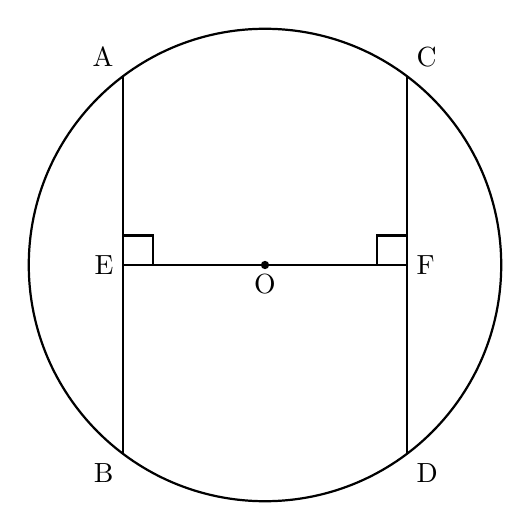
\begin{tikzpicture}[scale=1.5]

    % --- Define Coordinates ---
    % Origin/Center
    \coordinate (O) at (0,0);
    
    % Positions for vertical chords. 
    % Assuming radius is 2, and x-distance is 1.2
    % Calculation for y: sqrt(2^2 - 1.2^2) = 1.6
    \coordinate (E) at (-1.2, 0);
    \coordinate (F) at (1.2, 0);
    
    % Endpoints of Chord AB
    \coordinate (A) at (-1.2, 1.6);
    \coordinate (B) at (-1.2, -1.6);
    
    % Endpoints of Chord CD
    \coordinate (C) at (1.2, 1.6);
    \coordinate (D) at (1.2, -1.6);

    % --- Drawing the Geometry ---
    
    % Draw the main circle
    \draw[thick] (O) circle (2cm);

    % Draw the vertical chord AB on the left
    \draw[thick] (A) -- (B);

    % Draw the vertical chord CD on the right
    \draw[thick] (C) -- (D);

    % Draw the horizontal segment EF connecting the chords through the center
    \draw[thick] (E) -- (F);

    % Draw the center point
    \fill (O) circle (1pt);

    % --- Right Angle Symbols ---
    
    % Right angle at E (formed by segment AE and EO)
    % Drawing a small square manually
    \draw[thick] (-1.2, 0.25) -- (-0.95, 0.25) -- (-0.95, 0);

    % Right angle at F (formed by segment CF and FO)
    % Drawing a small square manually
    \draw[thick] (1.2, 0.25) -- (0.95, 0.25) -- (0.95, 0);

    % --- Labels ---
    
    % Label points exactly as shown in the image
    \node[above left] at (A) {A};
    \node[below left] at (B) {B};
    \node[above right] at (C) {C};
    \node[below right] at (D) {D};
    \node[left] at (E) {E};
    \node[right] at (F) {F};
    \node[below] at (O) {O};

\end{tikzpicture}

\end{document}